\documentclass{article}
\usepackage{graphicx}
\usepackage{amsmath}
\usepackage{listings}
\usepackage{xcolor}
\usepackage{hyperref}
\usepackage{listings}
\usepackage{fancyhdr}
\usepackage[a4paper, hmargin = 1.5cm, head = 4cm, bottom = 2cm]{geometry}

\pagestyle{fancy}
\lhead{\includegraphics[width=0.27\textwidth]{assets/eth_logo.pdf}}
\rhead{Systems Programming and Computer Architecture}
\lfoot{Autumn Semester 2022}
\rfoot{\thepage}
\cfoot{}
\renewcommand{\footrulewidth}{1pt}

\begin{document}

\begin{titlepage}
    \thispagestyle{fancy}
    \renewcommand{\headrulewidth}{1pt}

    \center
    \vspace*{1.0cm}
    \Large Systems Programming and Computer Architecture \\[.5 cm]
    \large
    \normalsize
    Gnkgo, Informatik B. Sc. 3. Semester \\
    \vfill
\end{titlepage}

% Table of Contents
\tableofcontents
\newpage % Start content on a new page



\section{Calculations}

\subsection{Nested Array Row}

\begin{verbatim}
arr[N][M]

arr[i][j] = arr + (i * M + j)
\end{verbatim}

\subsection{IEEE}

\textbf{Exp = 000 ... 0} $\rightarrow$ -Bias + 1, leading 0.

\subsection{Cache}

Each page table entry PTE contains only the PPN and the metadata

\textbf{With multilevel decoding, from virtual address to physical address} virtual address space - page offset = bits to be encoded. Bits to be encoded / levels

\textbf{Minimum size of each PTE in bytes} Physical address space - Pagesize + Flags(Metadata)

\textbf{Size of processor's page table} Virtual address space - pagesize + PTE size

\textbf{False Sharing} Poor performance when on different processors $\rightarrow$ flush whole cache even though they didn't need the same location. Good performance when on the same processor

\textbf{Number of misses} Two arrays map to the same cache line if the address \% cachesize is the same. Then you would have 100\% cache misses

\section{Parallel Programming}

\subsection{Solving ABA problem}

\begin{itemize}
    \item \textbf{Hazard Pointers:} Threads keep track of questioned pointers in a shared data structure. Each thread knows that the object on the given memory address defined by the pointer might have been modified by another thread.
    \item \textbf{Immutability:} The usage of immutable objects solves this problem, as we don't reuse objects across the application.
    \item \textbf{Double Compare and Swap:} Keep track of one more variable, which is the version number.
\end{itemize}

\section{Architecture}

\textbf{Section header table} Offsets and sizes of each section

\textbf{symtab.} Symbol table, procedure and static variable names, section names and locations

\textbf{.rel.text} Relocation info for .text section instructions for modifying

\textbf{.debug*} Info for symbolic debugging (gcc. -g)

It exists 1 virtual address space per process

\textbf{Metadata bits in PTE}
\begin{itemize}
    \item \textbf{D:} Dirty
    \item \textbf{A:} Accessed
    \item \textbf{P:} Page is present in physical memory (1) or not(0)
    \item \textbf{Avail:} Available for system programmers
\end{itemize}

\subsection{Memory}

Performance is \textit{not uniform}!
Cache and virtual memory effects can greatly affect program performance.

\textit{Typed}
Different kinds of memory behave differently.

\textit{Not unbounded}
It must be allocated and managed.

\textbf{Non-Uniform Memory Access (NUMA)} Removes bottleneck
\begin{itemize}
    \item Multiple, independent memory banks
    \item Processors have independent paths to memory
    \item Cannot snoop on the bus anymore $\rightarrow$ it's not a bus! Use a message-passing interconnect
\end{itemize}

Solution1: Bus emulation
\begin{itemize}
    \item Similar to snooping but without a shared bus
    \item Each node sends a message to all other nodes (e.g., read exclusive)
    \item Waits for a reply from all nodes before proceeding (e.g., acknowledge)
    \item \textit{AMD coherent HyperTransport}
\end{itemize}

Solution2: Cache Directory
\begin{itemize}
    \item Augment each node's local memory with a cache directory
\end{itemize}

\textbf{Directory-based Cache Coherence}
\begin{itemize}
    \item Home node maintains a set of nodes that may have line Large multiprocessors
    \item More efficient when:
    \begin{itemize}
        \item Lines are not widely shared
        \item Lots of NUMA nodes
        \item Avoid broadcast/incast
        \item Reduces interconnect traffic, load at each node
        \item Requires lots of fast memory
    \end{itemize}
\end{itemize}

\subsection{Locks}

\textbf{MCS locks}
\begin{itemize}
    \item \textit{Problem:} Cache line containing lock is a \textit{hot spot}
    \begin{itemize}
        \item Continuously invalidated as every processor tries to acquire it
        \item Dominates interconnect traffic
    \end{itemize}
    \item \textit{Solution:} When acquiring, a processor enqueues itself on a list of waiting processors, and spins on its \textit{own entry} in the list
\end{itemize}

\begin{verbatim}
struct qnode {
    struct qnode *next;
    int locked;
};
typedef struct qnode *lock_t;

void acquire(lock_t *lock, struct qnode *local) {
    local -> next = NULL;
    struct qnode *prev = XCHG(lock, local);
    if (prev) { // queue was non-empty
        local-> locked = 1;
        prev -> next = local;
        while (local -> locked); // spin
    }
}

void release(lock_t *lock, struct qnode *local) {
    if (local->next == NULL) {
        if (CAS(lock, local, NULL)) {
            return;
        }
        while(local->next ==NULL); // spin
    }
    local -> next -> locked = 0;
}
\end{verbatim}

\textbf{Flags}
\begin{figure}[h]
    \centering
    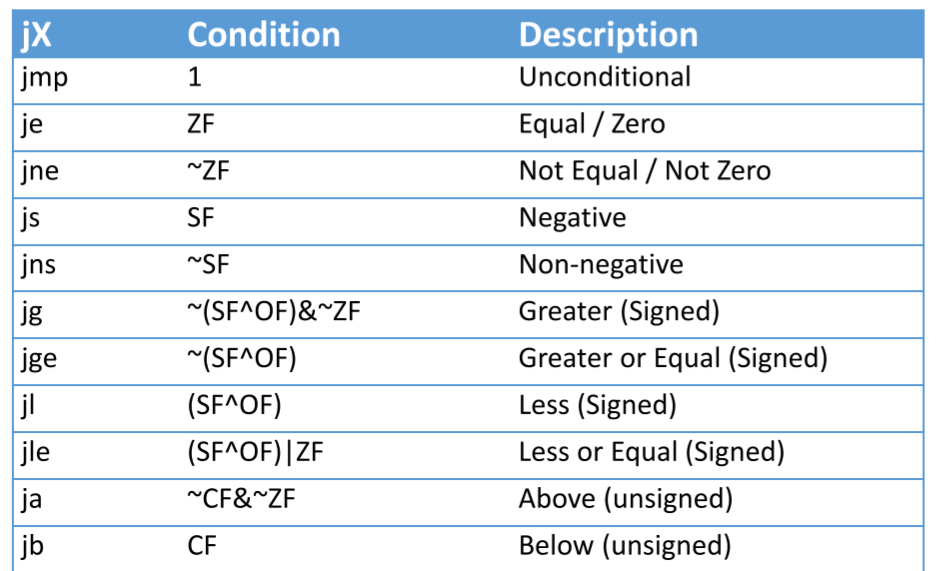
\includegraphics[width=0.5\textwidth]{flag_table.png}
    \caption{Flags Table}
\end{figure}

\textbf{Synonym}
\begin{itemize}
    \item Only in virtual part
    \item Different VAs map to the same PA
    \item VV with keys remove homonyms but create synonyms
\end{itemize}

\textbf{Homonym}
\begin{itemize}
    \item Same name for different data
    \item Same VA refers to different PAs
    \item Flush cache on context switch
    \item Force non-overlapping address-space
    \item Tag VA with address-space
\end{itemize}

\subsection{Jumps}

\textbf{Longjmp:} If retval = 0, longjmp returns 1

\textbf{Setjump:} Saves the current calling environment
\begin{itemize}
    \item Program counter (not necessary)
    \item Stack pointer
    \item General-purpose register
\end{itemize}

Or as it was mentioned in the exam:
\begin{itemize}
    \item Current stack pointer
    \item The current program counter (\%rip)
    \item Callee-save processor registers
    \item Frame pointer register §rbp
\end{itemize}

\subsection{MESI}

\begin{itemize}
    \item Dirty data always written through memory
    \item No cache cache transfer
    \item Good if latency of memory $<<$ latency of remote cache
\end{itemize}

\subsection{Program Order}

Order in which a program on a processor appears to issue reads and writes. Refers only to \textbf{local} reads/writes

\subsection{Visibility Order}

Order in which all reads and writes are seen by one or more processors. Refers to all operations in the machine

\subsection{Sequential Consistency}

Think of PPROG $\rightarrow$ Order is important but you can move instructions horizontally
\begin{enumerate}
    \item Operations from a processor appear (to all others) in program order
    \item Every processor's visibility order is the interleaving of all the program orders
\end{enumerate}

\textbf{Requirements:}
\begin{itemize}
    \item Each processor issues memory ops in program order
    \item Memory operations are atomic
\end{itemize}

\section{Dependence}

\textbf{Anti-dependence} write after read, can avoid hazard with register renaming

\textbf{Output-dependence} write after write, can avoid hazard with register renaming

\textbf{True-dependence} read after write

\subsection{Order on stack}

\textit{Extra args}

\textit{Return address}

\textit{Saved base pointer}

\textit{Local variables}

\section{Exceptions}

\textbf{Processor Exception} changes the control flow exceptionally and most of the time context switches to the OS for further instructions on how the given exception should be handled. Exceptions are associated with an exception code that at the same time is an index into an exception table defined by the OS. In contrast to, for example, Java exceptions, processor exceptions are not always bad; a system call is often handled as an exception too.

\textbf{Asynchronous exception} caused by events outside of the processor $\rightarrow$ ctrl-c (interrupt)

\textbf{Synchronous exception} caused by an instruction of the processor

\subsection{Abort}

\begin{itemize}
    \item Nonrecoverable error
    \item Sync
    \item Unintentional
    \item Machine check
    \item \textbf{Aborts current program}
\end{itemize}

\subsection{Fault}

\begin{itemize}
    \item Potentially recoverable error
    \item Sync
    \item Unintentional
    \item Page fault, protection fault
    \item \textbf{Either re-executes the faulting instruction or abort}
\end{itemize}

\subsection{Trap}

\begin{itemize}
    \item Intentional
    \item Sync
    \item System calls, breakpoint trap
    \item \textbf{Returns control to "next" instruction}
\end{itemize}

\section{Linker}

\begin{itemize}
    \item Resolving symbol references from other files
    \item Merging different object file sections
\end{itemize}

\section{Toolchain}

\textit{How C code turns into an executable file}

C source - Preprocessor - Compiler - Assembler - Linker - Executable

\textit{GNU gcc Toolchain}

CPP (Macro substitution include header files) - CC1 (compile each C file into assembly language) - as (Assemble each file into object code) - ld (link object files into program binary) - Executable

\section{Debugger}

\textbf{Valgrind} helpful for memory-related errors

\textbf{GDB} conventional debugger, good for finding bad pointer dereferences, hard to detect the other memory bugs

\textbf{Objdump} Useful tool for examining object code, analyzes the bit pattern of series of instructions

\section{Random}

\textbackslash\textbackslash is an escape.

\textit{PIC, Programmable Interrupt Controller}
\begin{itemize}
    \item Map physical interrupt pins to interrupt vectors
    \item Buffer simultaneous interrupts $\rightarrow$ Won't lose some device's interrupt
    \item Prioritize interrupts
    \item Selectively mask any individual device's interrupts useful for high interrupt rate
\end{itemize}

How many BxB blocks fit into a cache and how many blocks do you need? $\rightarrow$ $X B^2 < C$ where X is mostly 3 and C the Cache size

Reading a string of length 10 in the buffer
\begin{verbatim}
fgets(buf, 10, stdin);
fscanf(stdin, "%9s", buf);
\end{verbatim}

\begin{verbatim}
NULL = (void *) 0
\end{verbatim}

\begin{verbatim}
strncpy(char *dest, const char *source, size)
\end{verbatim}

DRAM as cache: Fully associative, sophisticated replacement policy, writeback

\begin{verbatim}
void print_integers(unsigned num_ints, char *msg, ...) {
    va_list ap; // Variable which keeps track of which argument we're currently looking at, a bit like an iterator
    va_start(ap, msg); // Initialize the iterator based on the last fixed argument;
    for (int i = 0; i < num_ints; i++>) {
        int j = va_arg(ap, int);//return the next argument, cast to an int
        printf("int %d = %d\n", i, j);
    }
    va_end(ap) //free up the iterator
}
\end{verbatim}

\end{document}
